% !TeX program = xelatex
% !TeX encoding = UTF-8
\documentclass{book}
% \usepackage{xeCJK}
\usepackage{amsmath,extarrows}
\let\lvert\relax\let\rvert\relax\let\lVert\relax\let\rVert\relax
\usepackage[upint]{newtxmath}
\usepackage{siunitx,physics}
\usepackage{ctex}
\usepackage{caption}
\usepackage{ctex}
\usepackage[a4paper,textheight = 550pt,textwidth = 360pt,marginparwidth=5cm,inner=3cm,top=2.5cm,bottom=2.5cm]{geometry}
\usepackage{layout}
\usepackage{titlesec}
\newcommand{\secformat}[1]{\MakeLowercase{\so{#1}}}
\titleformat{\section}[block]
{\normalfont\scshape\filcenter}
{\thesection}
{1em}
{\secformat}
\titleformat{\section}[leftmargin]
{\normalfont
\titlerule*[.6em]{\bfseries.}%
\vspace{6pt}%
\sffamily\bfseries\filleft}
{\thesection}{.5em}{}
\titlespacing{\section}
{6pc}{1.5ex plus .1ex minus .2ex}{1pc}
\usepackage{ntheorem}
{
	\theoremstyle{change}
	\theoremheaderfont{\bfseries}
	\theorembodyfont{\normalfont}
	\newtheorem{ti}{}[section]
}
\renewcommand{\theti}{\arabic{ti}.}
{
	\theoremstyle{nonumberplain}
	\theoremheaderfont{\bfseries}
	\theorembodyfont{\itshape}
	\newtheorem{solution}{解}
}
\let\div\relax\let\grad\relax
\DeclareMathOperator{\div}{div}
\DeclareMathOperator{\grad}{grad}
\DeclareMathOperator{\rot}{rot}
% \def\frac{\dfrac}
% \def\frac{\tfrac}
\def\partial{\uppartial}
\def\ee{\mathrm{e}}
\def\theenumi{\arabic{enumi}}
\def\labelenumi{(\theenumi)}
\title{《工程电磁场》复习重点及历年真题}
\author{死抠}
\usepackage{tikz}
\usepackage{hyperref}
\begin{document}
\frontmatter
\maketitle
\tableofcontents
\mainmatter
% \layout
\chapter{知识点总结}
\section{矢量分析与场论思想}
\raggedright 重点为:方向导数、梯度、散度、环量、旋度、散度定理、斯托克斯定理的计算
\begin{ti}[方向导数]
	\[
		\frac{\dd u}{\dd l}=\frac{\partial u}{\partial x}\cos \alpha+\frac{\partial u}{\partial y}\cos \beta+\frac{\partial u}{\partial z}\cos \gamma
	\]
	其中 $\cos \alpha=\frac{\dd x}{\dd l}$,$\cos \beta=\frac{\dd y}{\dd l}$,$\cos \gamma=\frac{\dd z}{\dd l}$。
\end{ti}

\begin{ti}[梯度]
	\[
		\grad u=\frac{\partial u}{\partial x}\vec e_x+\frac{\partial u}{\partial y}\vec e_x+\frac{\partial u}{\partial z}\vec e_z
	\]
	其中梯度的运算与微分运算类似,这里不再赘述。
\end{ti}

\begin{ti}[散度]
	\[
		\div\vec A=\frac{\partial A_x}{\partial x}+\frac{\partial A_y}{\partial y}+\frac{\partial A_z}{\partial z}
	\]
	散度的运算公式
	\begin{enumerate}
		\item $\div(C\vec{A})=C\div\vec{A}$
		\item $\div(u\vec{A})=u\div\vec{A}+\grad u\bullet\vec{A}$
		\item $\div(\vec{A}\pm\vec{B})=\div\vec{A}\pm\div\vec{B}$
	\end{enumerate}
	散度定理
	\[
		\oiint_{S}{\vec{A}\cdot\dd \vec{S}}=\iiint_{V}{\div\vec{A}\dd V}
	\]
\end{ti}

\begin{ti}[旋度]
	\[
	\rot\vec{A}=
	\begin{vmatrix}
	\vec e_x&\vec e_y&\vec e_z\\
	\frac{\partial}{\partial x}&\frac{\partial}{\partial y}&\frac{\partial}{\partial z}\\
	A_x&A_y&A_z
	\end{vmatrix}
	\]
	旋度的运算公式
	\begin{enumerate}
		\item $\rot(C\vec{A})=C\rot\vec{A}$
		\item $\rot(\vec{A}\pm\vec{B})=\rot\vec{A}\pm\rot\vec{B}$
		\item $\rot(u\vec{A})=u\rot\vec{A}+\grad u\times\vec{A}$
		\item $\rot(\grad u)=0$(重要的矢量恒等式)
		\item $\div(\vec{A}\times\vec{B})=\vec{B}\bullet\rot\vec{A}-\vec{A}\bullet\rot\vec{B}$
		\item $\div(\rot\vec{A})=0$(重要的矢量恒等式)
	\end{enumerate}
	斯托克斯定理
	\[
		\oint_l{\vec{A}\bullet\dd \vec{l}}=\iint_S{\rot\vec{A}\bullet\dd \vec{S}}
	\]
\end{ti}

\begin{ti}[哈密尔顿(纳布拉)算子]
	\[
		\bigtriangledown=\vec{e}_x\frac{\partial}{\partial x}+\vec{e}_y\frac{\partial}{\partial y}+\vec{e}_z\frac{\partial}{\partial z}
	\]
	因此,梯度
	\[
		\grad u=\frac{\partial u}{\partial x}\vec{e}_x+\frac{\partial u}{\partial y}\vec{e}_y+\frac{\partial u}{\partial z}\vec{e}_z=\bigtriangledown u
	\]
	散度
	\[
		\div\vec A=\frac{\partial A_x}{\partial x}+\frac{\partial A_y}{\partial y}+\frac{\partial A_z}{\partial z}=\bigtriangledown\bullet\vec{A}
	\]
	旋度
	\[
		\rot\vec{A}=
	\begin{vmatrix}
	\vec e_x&\vec e_y&\vec e_z\\
	\frac{\partial}{\partial x}&\frac{\partial}{\partial y}&\frac{\partial}{\partial z}\\
	A_x&A_y&A_z
	\end{vmatrix}=\bigtriangledown\times\vec{A}
	\]
	拉普拉斯算子
	\[
		\bigtriangledown^2=\bigtriangledown\bullet\bigtriangledown=\frac{\partial^2}{\partial x^2}+\frac{\partial^2}{\partial y^2}+\frac{\partial^2}{\partial z^2}
	\]
	$\bigtriangledown$ 算子常用运算公式
	\begin{enumerate}
		\item 散度定理
		\[
			\iiint_{V}{\bigtriangledown\bullet\vec{A}}\dd V=\oiint_{S}{\vec{A}\bullet\dd \vec{S}}
		\]
		\item 斯托克斯定理
		\[
			\iint_S{\bigtriangledown\times\vec{A}\bullet\dd \vec{S}}=\oint_l{\vec{A}\bullet\dd \vec{l}}
		\]
	\end{enumerate}
\end{ti}

\begin{ti}[常用坐标系中的有关公式]
	拉梅系数
	\[
		h_u,h_v,h_w
	\]
	若
	\[
		\dd \vec{l}=h_u\dd \vec{u}+h_v\dd \vec{v}+h_w\dd \vec{w}
	\]
	则有
	\[
		\bigtriangledown a=\frac1{h_u}\frac{\partial a}{\partial u}\vec{e}_u+\frac1{h_v}\frac{\partial a}{\partial v}\vec{e}_v+\frac1{h_w}\frac{\partial a}{\partial w}\vec{e}_w
	\]
	\[
		\bigtriangledown\bullet\vec{A}=\frac{1}{h_uh_vh_w}\left[\frac{\partial}{\partial u}(A_uh_vh_w)+\frac{\partial}{\partial v}(A_vh_uh_w)+\frac{\partial}{\partial w}(A_wh_uh_v)\right]
	\]
	\[
		\bigtriangledown\times\vec{A}=\frac{1}{h_uh_vh_w}
	\begin{vmatrix}
	h_u\vec{e}_u&h_v\vec{e}_v&h_w\vec{e}_w\\
	\frac{\partial}{\partial u}&\frac{\partial}{\partial v}&\frac{\partial}{\partial w}\\
	h_uA_u&h_vA_v&h_wA_w
	\end{vmatrix}
	\]
	那么在柱面坐标系中有
	\[
		\dd \vec{l}=\dd \vec{r}+r\dd \vec{\alpha}+\dd \vec{z}
	\]
	即
	\[
		h_u=1,h_v=r,h_w=1
	\]
	那么在球面坐标系中有
	\[
		\dd \vec{l}=\dd \vec{r}+r\dd \vec{\theta}+r\sin\theta\dd \vec{\alpha}
	\]
	即
	\[
		h_u=1,h_v=r,h_w=r\sin\theta
	\]
\end{ti}

\section{静电场的基本原理}
重点为:电场强度、电位移矢量、极化强度、极化电荷体密度、极化电荷面密度的计算,电位与电场强度的关系,衔接条件
\begin{ti}[电场强度]
\[
	E=\frac{q}{4\uppi\varepsilon_0R^2}\vec{e}_R
\]
电荷线密度
\[
	\tau=\frac{\dd q}{\dd l}
\]
电荷面密度
\[
	\sigma=\frac{\dd q}{\dd S}
\]
电荷体密度
\[
	\rho=\frac{\dd q}{\dd V}
\]
线电荷产生的电场强度
\[
	E=\frac{1}{4\uppi\varepsilon_0}\int_l{\frac{\tau\vec{e}_R}{R^2}}\dd l
\]
面电荷产生的电场强度
\[
	E=\frac{1}{4\uppi\varepsilon_0}\iint_S{\frac{\sigma\vec{e}_R}{R^2}}\dd S
	\]
体电荷产生的电场强度
\[
	E=\frac{1}{4\uppi\varepsilon_0}\iiint_{V}{\frac{\rho\vec{e}_R}{R^2}}\dd V
\]
\end{ti}

\begin{ti}[电位]
\[
	\varphi=\frac{1}{4\uppi\varepsilon_0}\iiint_{V}\frac{\rho}{R}\dd V+C
\]
面、线情况下的电位不再赘述,电位与电场强度的关系
\[
	E=-\bigtriangledown\varphi
\]
静电场环路定理的微分形式
\[
	\bigtriangledown\times\vec{E}=0
\]
静电场环路定理的积分形式
\[
	\oint_l{E\bullet\dd \vec{l}}=0
\]
高斯通量定理的微分形式
\[
	\bigtriangledown\bullet \vec{E}=\frac{\rho}{\varepsilon_0}
\]
高斯通量定理的积分形式
\[
	\oiint_{S}\vec{E}\bullet\dd \vec{S}=\iiint_{V}{\bigtriangledown\bullet\vec{E}}\dd V=\iiint_{V}{\frac{\rho}{\varepsilon_0}}\dd V=\frac{q}{\varepsilon_0}
\]
\end{ti}

\begin{ti}[电位移矢量]
\[
	\vec{D}=\varepsilon_0\vec{E}+\vec{P}
\]
其中 $\vec{P}$ 为极化强度,极化电荷体密度
\[
	\rho_P=-\bigtriangledown\bullet\vec{P}
\]
极化电荷面密度
\[
	\sigma_P=\vec{P}\bullet\vec{e}_\mathrm{n}
\]
高斯通量定理的微分形式
\[
	\bigtriangledown\bullet\vec{D}=\rho
\]
高斯通量定理的积分形式
\[
	\oiint_{S}\vec{D}\bullet\dd \vec{S}=\iiint_{V}{\bigtriangledown\bullet\vec{D}}\dd V=q
\]
\end{ti}

\begin{ti}[静电场的辅助方程]
在各向同性的介质中
\[
	\vec{D}=\varepsilon\vec{E}
\]
\end{ti}

\begin{ti}[静电场的基本方程与分界面衔接条件]
静电场基本方程
\[
\begin{matrix}
\text{微分形式}&\text{积分形式}\\
\bigtriangledown\times\vec{E}=0&\oint_l{\vec{E}\bullet\dd \vec{l}}=0\\
\bigtriangledown\bullet\vec{D}=\rho&\oiint_{S}{\vec{D}\bullet\dd \vec{S}}=q
\end{matrix}
\]
辅助方程为
\[
	\vec{D}=\varepsilon\vec{E}
\]
电介质分界面条件
\[
	\vec{e}_{\mathrm{n}}\times(\vec{E}_2-\vec{E}_1)=0\Leftrightarrow E_{2\text{t}}=E_{1\text{t}}
\]
\[
	\vec{e}_\mathrm{n}\bullet(\vec{D}_2-\vec{D}_1)=\sigma\Leftrightarrow D_{2\mathrm{n}}-D_{1\mathrm{n}}=\sigma
\]
\end{ti}

\section{恒定电场的基本原理}
重点为:电流密度与电场强度的关系,电流密度的计算,衔接条件
\begin{ti}[电流密度]
\[
	 J=\rho v=\rho\frac{\dd l}{\dd t}=\frac{\rho\dd S_0\dd l}{\dd t\dd S_0}=\frac{\rho\dd V}{\dd t\dd S_0}=\frac{\dd q}{\dd t\dd S_0}=\frac{\dd I}{\dd S_0}
\]
电流密度与电场强度的关系
\[
	\vec{J}=\gamma\vec{E}\Leftrightarrow\vec{E}=\frac{1}{\gamma}\vec{J}=\rho_R\vec{J}
\]
\end{ti}

\begin{ti}[电动势]
\[
	e=\int_{a}^{b}{E_{\ee }\bullet\dd \vec{l}}
\]
\end{ti}

\begin{ti}[电流连续性]
电荷守恒原理的积分形式
\[
	\oiint_{S}{\vec{J}\bullet\dd \vec{S}}=-\frac{\partial q}{\partial t}
\]
电荷守恒原理的微分形式
\[
	\bigtriangledown\bullet\vec{J}=-\frac{\partial\rho}{\partial t}
\]
对于恒定电场(即 $\frac{\partial\rho}{\partial t}=0,\frac{\partial q}{\partial t}=0$ )有恒定电场的电流连续性方程
\begin{gather*}
	\bigtriangledown\bullet\vec{J}=0\\
	\oiint_{S}{J\bullet\dd \vec{S}}=0
\end{gather*}
\end{ti}

\begin{ti}[恒定电场的基本方程及辅助方程]
恒定电场的基本方程
\[
\begin{matrix}
\text{微分形式}&\text{积分形式}\\
\bigtriangledown\bullet\vec{J}=0&\oiint_{S}{\vec{J}\bullet\dd \vec{S}}=0\\
\bigtriangledown\times\vec{E}=0&\oint_l{\vec{E}\bullet\dd \vec{l}}=0
\end{matrix}
\]
辅助方程为
\[
	\vec{J}=\gamma\vec{E}
\]
在均匀媒质中,电位的基本方程
\[
	\gamma\bigtriangledown^2\varphi=0
\]
\end{ti}

\begin{ti}[导电媒质分界面衔接条件]
\begin{gather*}
	\vec{e}_{\mathrm{n}}\times(\vec{E}_2-\vec{E}_1)=0\Leftrightarrow E_{2\text{t}}=E_{1\text{t}}\\
	\vec{e}_\mathrm{n}\bullet(\vec{J}_2-\vec{J}_1)=0\Leftrightarrow J_{2\mathrm{n}}=J_{1\mathrm{n}}
\end{gather*}
将
\[
	\vec{E}=-\bigtriangledown\varphi,\vec{J}=\gamma\vec{E}
\]
代入上述分界面条件,得到电位应满足的分界面衔接条件
\[
\begin{cases}
\varphi_1=\varphi_2\\
\gamma_2\frac{\partial\varphi_2}{\partial n}=\gamma\frac{\partial\varphi_1}{\partial n}
\end{cases}
\]
\end{ti}

\section{恒定磁场的基本原理}
重点为:用安培环路定理($2$ 种)计算磁感应强度、磁场强度
\begin{ti}[毕奥-沙伐定律]
\[
	\vec{B}=\frac{\mu_0}{4\uppi}\oint_l{\frac{I\dd \vec{l}\times\vec{e}_R}{R^2}}\Leftrightarrow\dd \vec{B}=\frac{\mu_0}{4\uppi}\frac{I\dd \vec{l}\times\vec{e}_R}{R^2}
\]
\end{ti}

\begin{ti}[分布电流的磁感应强度]
点电流
\[
	\vec{B}=\frac{\mu_0}{4\uppi}\frac{q\vec{v}\times\vec{e}_R}{R^2}
\]
线电流
\[
	\vec{B}=\frac{\mu_0}{4\uppi}\oint_l\frac{I\dd l\times\vec{e}_R}{R^2}
\]
面电流
\[
	\vec{B}=\frac{\mu_0}{4\uppi}\iint_S\frac{\vec{K}\times\vec{e}_R}{R^2}\dd S
\]
体电流
\[
	\vec{B}=\frac{\mu_0}{4\uppi}\iiint_{V}\frac{\vec{J}\times\vec{e}_R}{R^2}\dd V
\]
\end{ti}

\begin{ti}[洛伦兹力]
\[
	\vec{F}=q\vec{v}\times\vec{B}
\]
\end{ti}

\begin{ti}[磁通连续性定理]
\[
\begin{matrix}
\text{微分形式}&\text{积分形式}\\
\bigtriangledown\bullet\vec{B}=0&\oiint_{S}{\vec{B}\bullet\dd \vec{S}}=0
\end{matrix}
\]
\end{ti}

\begin{ti}[安培环路定理]
\[
	\begin{matrix}
	\text{微分形式}&\text{积分形式}\\
	\bigtriangledown\times\vec{B}=\mu_0\vec{J}&\oint_l{\vec{B}\bullet\dd \vec{l}}=\mu_0I
	\end{matrix}
\]
\end{ti}

\begin{ti}[磁场强度]
\[
	\vec{H}=\frac{\vec{B}}{\mu_0}-\vec{M}
\]
其中 $\vec{M}$ 为磁化强度,安培环路定理
\[
	\begin{matrix}
	\text{微分形式}&\text{积分形式}\\
	\bigtriangledown\times\vec{H}=\vec{J}&\oint_l{\vec{H}\bullet\dd \vec{l}}=I
	\end{matrix}
\]
\end{ti}

\begin{ti}[恒定磁场的基本方程与分界面衔接条件]
恒定磁场的基本方程
\[
	\begin{matrix}
	\text{微分形式}&\text{积分形式}\\
	\bigtriangledown\bullet\vec{B}=0&\oiint_{S}{\vec{B}\bullet\dd \vec{S}}=0\\
	\bigtriangledown\times\vec{H}=\vec{J}&\oint_l{\vec{H}\bullet\dd \vec{l}}=I
	\end{matrix}
\]
辅助方程为
\[
	\vec{B}=\mu\vec{H}
\]
媒质分界面的衔接条件
\begin{gather*}
	\vec{e}_{\mathrm{n}}\times(\vec{H}_2-\vec{H}_1)=\vec{K} \\
	\vec{e}_{\mathrm{n}}\bullet(\vec{B}_2-\vec{B}_1)=0\Leftrightarrow B_{2\mathrm{n}}=B_{1\mathrm{n}}
\end{gather*}
其中 $\vec{K}$ 为分界面的自由面电流密度
\end{ti}

\section{时变电磁场的基本原理}
重点为:位移电流、全电流( $\vec{J}_\text{C},\frac{\partial\vec{D}}{\partial t}$ 是重点)的计算
\begin{ti}[时变场中的运动回路]
电磁感应定律
\[
	\begin{matrix}
	\text{微分形式}&\text{积分形式}\\
	\bigtriangledown\times\vec{E}=-\frac{\partial\vec{B}}{\partial t}+\bigtriangledown\times(\vec{v}\times\vec{B})&
	\oint_l{\vec{E}\bullet\dd \vec{l}}=-\iint_S{\frac{\partial\vec{B}}{\partial t}}\bullet\dd \vec{S}+\oint_l{(\vec{v}\times\vec{B})}\bullet\dd \vec{l}
	\end{matrix}
\]
\end{ti}

\begin{ti}[时变场的电流连续性]
\[
	\bigtriangledown\bullet\left(\vec{J}_C+\frac{\partial\vec{D}}{\partial t}\right)=0
\]
\end{ti}

\begin{ti}[全电流定律]
\[
	\begin{matrix}
	\text{微分形式}&\text{积分形式}\\
	\bigtriangledown\times\vec{H}=\vec{J}_\text{C}+\vec{J}_v+\frac{\partial\vec{D}}{\partial t}&\oint_l{\vec{H}\bullet\dd \vec{l}}=i_\text{C}+i_{\dd}+i_v
	\end{matrix}
\]
\end{ti}

\begin{ti}[电磁场的基本方程组]
\[
	\begin{matrix}
	\text{微分形式}&\text{积分形式}\\
	\bigtriangledown\times\vec{H}=\vec{J}_\text{C}+\rho\vec{v}+\frac{\partial\vec{D}}{\partial t}&\oint_l{\vec{H}\bullet\dd \vec{l}}=\iint_S{\vec{J}_\text{C}\bullet\dd \vec{S}}+\iint_S{\rho\vec{v}\bullet\dd \vec{S}}+\iint_S{\frac{\partial\vec{D}}{\partial t}\bullet\dd \vec{S}}\\
	\bigtriangledown\times\vec{E}=-\frac{\partial\vec{B}}{\partial t}&\oint_l{\vec{E}\bullet\dd \vec{l}}=-\iint_S{\frac{\partial\vec{B}}{\partial t}\bullet\dd \vec{S}}\\
	\bigtriangledown\bullet\vec{B}=0&\oiint_{S}{\vec{B}\bullet\dd \vec{S}}=0\\
	\bigtriangledown\bullet\vec{D}=\rho&\oiint_{S}{\vec{D}\bullet\dd \vec{S}}=q
	\end{matrix}
\]
在各向同性媒质中,辅助方程为
\begin{align*}
	\vec{D}&=\varepsilon\vec{E},\\
	\vec{B}&=\mu\vec{H},\\
	\vec{J}_\text{C}&=\gamma\vec{E}
\end{align*}
媒质分界面衔接条件
\[
\begin{matrix}
\vec{e}_{\mathrm{n}}\bullet(\vec{D}_2-\vec{D}_1)=\sigma&\vec{e}_\mathrm{n}\bullet(\vec{B}_2-\vec{B}_1)=0\\
\vec{e}_\mathrm{n}\times(\vec{E}_2-\vec{E}_1)=0&\vec{e}_\mathrm{n}\times(\vec{H}_2-\vec{H}_1)=\vec{K}
\end{matrix}
\]
\end{ti}

\chapter{重点习题}
\section{课后习题}
1-6,1-9,1-14,1-16,1-21,1-22,1-24,2-5,2-6,2-7,2-10,2-13,2-15,2-16,3-1,4-7,4-8,4-10,5-4,5-5,5-7,5-8,5-13

\section{书中例题}
设跨步电压安全限值为 $U_0$,入地电流为 $I$,试确定课本 $78$ 页图 3-4-6 所示的浅埋半球接地体附近地面的危险区

\chapter{历年真题}
\section{试卷编号:1819010634C}
\begin{ti}[10 分]
	求函数 $\varphi=xyz$ 在点 $(5,2,1)$ 处沿着点 $(5,1,2)$ 到 $(9,4,19)$ 方向的方向导数。
\end{ti}

\begin{ti}[10 分]
	已知标量场 $u=\ee ^x\sin y$,求 $\bigtriangledown u$。
\end{ti}

\begin{ti}[10 分]
	已知 $\vec{A}=xy^2z\vec{r}(\vec{r}=x\vec{e}_x+y\vec{e}_y+z\vec{e}_z)$,求 $\div \vec{A}$ 在 $M(3,3,2)$ 处的值。
\end{ti}

\begin{ti}[10 分]
	已知 $\vec{A}=xz^3\vec{e}_x-2x^2yz\vec{e}_y+2yz^4\vec{e}_z$,求 $\vec{A}$ 在 $M(1,-1,-1)$ 点的旋度。
\end{ti}

\begin{ti}[10 分]
	一个半径为 $a$ 的无限长圆柱,圆柱表面均匀分布面电荷密度 $\rho_S$,求圆柱面内、外的电场强度。
\end{ti}

\begin{ti}[10 分]
	给定平行板电容器的尺寸、电介质的介电常数,如图~\ref{fig:1} 所示,给定极板总电荷量下,求电容器中的电场强度。
	\marginpar{%
		\centering
		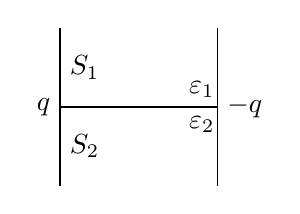
\begin{tikzpicture}
			\draw (0,0) ++ (0,-1) -- ++(0,2);
			\draw (0,0) -- ++ (2,0) ++ (0,-1) -- ++ (0,2);
			\node[left] at (0,0) {$q$};
			\node[right] at (2,0) {$-q$};
			\node[right] at (0,0.5) {$S_{1}$};
			\node[right] at (0,-0.5) {$S_{2}$};
			\node[above] at (1.8,0) {$\varepsilon_{1}$};
			\node[below] at (1.8,0) {$\varepsilon_{2}$};
		\end{tikzpicture}
		\captionof{figure}{}\label{fig:1}
	}
	% \begin{figure}[htbp]
	% 	\centering
	% 	\begin{tikzpicture}
	% 		\draw (0,0) ++ (0,-1) -- ++(0,2);
	% 		\draw (0,0) -- ++ (2,0) ++ (0,-1) -- ++ (0,2);
	% 		\node[left] at (0,0) {$q$};
	% 		\node[right] at (2,0) {$-q$};
	% 		\node[right] at (0,0.5) {$S_{1}$};
	% 		\node[right] at (0,-0.5) {$S_{2}$};
	% 		\node[above] at (1.8,0) {$\varepsilon_{1}$};
	% 		\node[below] at (1.8,0) {$\varepsilon_{2}$};
	% 	\end{tikzpicture}
	% 	\caption{}\label{fig:1}
	% \end{figure}
\end{ti}

\begin{ti}[15 分]
	如图~\ref{fig:2} 所示,试确定浅埋半球接地体的危险半径 $r_0$,设跨步电压安全限值为 $U_0$,入地电流为 $I$,土壤的电导率为 $\gamma$,跨步距离为 $b$。
	\marginpar{%
		\centering
		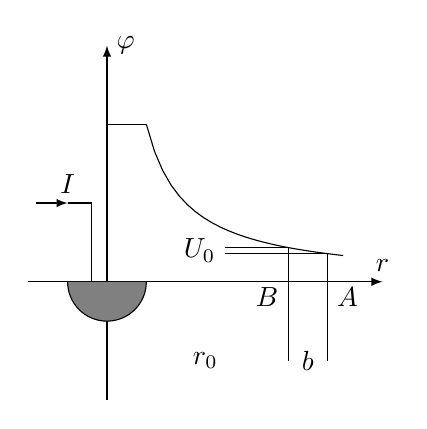
\begin{tikzpicture}[domain=0.5:3]
			\draw[-latex] (-1,0) -- (3.5,0) node[above] {$r$};
			\draw[-latex] (0,-1.5) -- (0,3) node[right] {$\varphi$};
			\filldraw[fill=gray,draw=black] (0.5,0) arc (0:-180:0.5) -- (-0.5,0);
			\draw[-latex] (-0.9,1) -- (-0.5,1) node[above] {$I$};
			\draw (-0.5,1) -- (-0.2,1) -- (-0.2,0);
			\draw (0,2) -- (0.5,2);
			\draw plot (\x,1/\x);
			\draw (1.5,1/2.3) -- (2.3,1/2.3) -- (2.3,-1);
			\draw (1.5,1/2.8) -- (2.8,1/2.8) -- (2.8,-1);
			\node[left] at (1.5,0.39596) {$U_{0}$};
			\node[left] at (2.3,-0.2) {$B$};
			\node[right] at (2.8,-0.2) {$A$};
			\node at (2.55,-1) {$b$};
			\node at (1.25,-1) {$r_{0}$};
		\end{tikzpicture}
		\captionof{figure}{}\label{fig:2}
	}
	% \begin{figure}[htbp]
	% 	\centering
	% 	\begin{tikzpicture}[domain=0.5:3]
	% 		\draw[-latex] (-1,0) -- (3.5,0) node[above] {$r$};
	% 		\draw[-latex] (0,-1.5) -- (0,3) node[right] {$\varphi$};
	% 		\filldraw[fill=gray,draw=black] (0.5,0) arc (0:-180:0.5) -- (-0.5,0);
	% 		\draw[-latex] (-0.9,1) -- (-0.5,1) node[above] {$I$};
	% 		\draw (-0.5,1) -- (-0.2,1) -- (-0.2,0);
	% 		\draw (0,2) -- (0.5,2);
	% 		\draw plot (\x,1/\x);
	% 		\draw (1.5,1/2.3) -- (2.3,1/2.3) -- (2.3,-1);
	% 		\draw (1.5,1/2.8) -- (2.8,1/2.8) -- (2.8,-1);
	% 		\node[left] at (1.5,0.39596) {$U_{0}$};
	% 		\node[left] at (2.3,-0.2) {$B$};
	% 		\node[right] at (2.8,-0.2) {$A$};
	% 		\node at (2.55,-1) {$b$};
	% 		\node at (1.25,-1) {$r_{0}$};
	% 	\end{tikzpicture}
	% 	\caption{}\label{fig:2}
	% \end{figure}
\end{ti}

\begin{ti}[10 分]
	如图~\ref{fig:3} 所示,已知无穷长电流和两种媒质的磁导率,求两种媒质中的磁感应强度。
	\marginpar{%
		\centering
		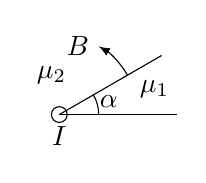
\begin{tikzpicture}
			\draw (0,0) node[below=1pt] {$I$} circle (0.1);
			\draw (0,0) -- ++ (1.5,0);
			\draw (0,0) -- ++ (30:1.5);
			\node at (15:1.25) {$\mu_{1}$};
			\draw (0.5,0) arc (0:30:0.5);
			\node at (15:0.65) {$\alpha$};
			\node at (-0.1,0.5) {$\mu_{2}$};
			\draw[-latex] (30:1) arc (30:60:1) node[left] {$B$};
		\end{tikzpicture}
		\captionof{figure}{}\label{fig:3}
	}
	% \begin{figure}[htbp]
	% 	\centering
	% 	\begin{tikzpicture}
	% 		\draw (0,0) node[below=1pt] {$I$} circle (0.1);
	% 		\draw (0,0) -- ++ (1.5,0);
	% 		\draw (0,0) -- ++ (30:1.5);
	% 		\node at (15:1.25) {$\mu_{1}$};
	% 		\draw (0.5,0) arc (0:30:0.5);
	% 		\node at (15:0.65) {$\alpha$};
	% 		\node at (-0.1,0.5) {$\mu_{2}$};
	% 		\draw[-latex] (30:1) arc (30:60:1) node[left] {$B$};
	% 	\end{tikzpicture}
	% 	\caption{}\label{fig:3}
	% \end{figure}
\end{ti}

\begin{ti}[15 分]
	一个球形电容器的内、外半径分别为 $a$ 和 $b$,内、外导体间材料的介电常数为 $\varepsilon$、电导率为 $\gamma$,在内、外导体间加低频电压 $u=U_m\cos\omega t$。求内外导体间的全电流。
\end{ti}




\chapter{历年真题参考答案}
\section{试卷编号:1819010634C}
\begin{ti}[10 分]
	求函数 $\varphi=xyz$ 在点 $(5,2,1)$ 处沿着点 $(5,1,2)$ 到 $(9,4,19)$ 方向的方向导数。
	\begin{solution}
		\[
			\bigtriangledown\varphi\left|_{(5,2,1)}\right.=(yz\vec{e}_x+xz\vec{e}_y+xy\vec{e}_z)\left|_{(5,2,1)}\right.=2\vec{e}_x+5\vec{e}_y+10\vec{e}_z
		\]
		沿着点 $(5,1,2)$ 到 $(9,4,19)$ 方向的单位矢量为
		\[
			\vec{a}=\frac{4\vec{e}_x+3\vec{e}_y+17\vec{e}_z}{\sqrt{4^2+3^2+17^2}}=\frac{4}{\sqrt{314}}\vec{e}_x+\frac{3}{\sqrt{314}}\vec{e}_y+\frac{17}{\sqrt{314}}\vec{e}_z
		\]
		则函数 $\varphi=xyz$ 在点 $(5,2,1)$ 处沿着点 $(5,1,2)$ 到 $(9,4,19)$ 方向的方向导数为
		\[
			\bigtriangledown\varphi\left|_{(5,2,1)}\right.\bullet\vec{a}=\frac{193}{\sqrt{314}}
		\]
	\end{solution}
\end{ti}

\begin{ti}[10 分]
	已知标量场 $u=\ee ^x\sin y$,求 $\bigtriangledown u$。
	\begin{solution}
		\[
		\bigtriangledown u = \frac{\partial u}{\partial x}\vec{e}_x+\frac{\partial u}{\partial y}\vec{e}_y
		= \ee ^x\sin y\vec{e}_x+\ee ^x\cos y\vec{e}_y
		\]
	\end{solution}
\end{ti}

\begin{ti}[10 分]
	已知 $\vec{A}=xy^2z\vec{r}(\vec{r}=x\vec{e}_x+y\vec{e}_y+z\vec{e}_z)$,求 $\div \vec{A}$ 在 $M(3,3,2)$ 处的值。
	\begin{solution}
		\[
			\vec{A}=x^2y^2z\vec{e}_x+xy^3z\vec{e}_y+xy^2z^2\vec{e}_z
		\]
		则
		\begin{align*}
			\left.\div \vec A\right|_M&= \left.\left(\frac{\partial A_x}{\partial x}+\frac{\partial A_y}{\partial y}+\frac{\partial A_z}{\partial z}\right)\right|_M\\
			&= \left.\left(2xy^2z+3xy^2z+2xy^2 z\right)\right|_M\\
			&= 378
		\end{align*}
	\end{solution}
\end{ti}

\begin{ti}[10 分]
	已知 $\vec{A}=xz^3\vec{e}_x-2x^2yz\vec{e}_y+2yz^4\vec{e}_z$,求 $\vec{A}$ 在 $M(1,-1,-1)$ 点的旋度。
	\begin{solution}
		\begin{align*}
			\left.\bigtriangledown\times\vec{A}\right|_M &= \left.
			\begin{vmatrix}
			\vec{e}_x & \vec{e}_y & \vec{e}_z\\
			\frac{\partial}{\partial x} & \frac{\partial}{\partial y} & \frac{\partial}{\partial z}\\
			xz^3 & -2x^2yz & 2yz^4
			\end{vmatrix}\right|_M
			=\left.\left(2z^4+2x^2y\right)\vec{e}_x+3xz^2\vec{e}_y-4xyz\vec{e}_z\right|_M\\
			&= 3\vec{e}_y-4\vec{e}_z
		\end{align*}
	\end{solution}
\end{ti}

\begin{ti}[10 分]
	一个半径为 $a$ 的无限长圆柱,圆柱表面均匀分布面电荷密度 $\rho_S$,求圆柱面内、外的电场强度。
	\begin{solution}
		在无限长圆柱轴线上作一以轴线为中心,半径为 $r$,高为 $h$ 的高斯圆柱面,设 $\vec{E}_r$ 为沿半径方向的电场强度
		
		当 $r<a$ 时,根据高斯通量定理,显然有 $\vec{E}_r=0$
		
		当 $r\geqslant a$ 时,根据对称性,上下面的电场强度为 $0$,根据高斯通量定理
		\[
			\oiint_{S}\vec{E}\dd \vec{S}=2\uppi\vec{E}_rrh=\frac{2\uppi ah\rho_S}{\varepsilon_0}
		\]
		即
		\[
			\vec{E}_r=\frac{a\rho_S}{r\varepsilon_0}
		\]
	\end{solution}
\end{ti}

\begin{ti}[10 分]
	给定平行板电容器的尺寸、电介质的介电常数,如图~\ref{fig:4} 所示,给定极板总电荷量下,求电容器中的电场强度。
	\marginpar{%
		\centering
		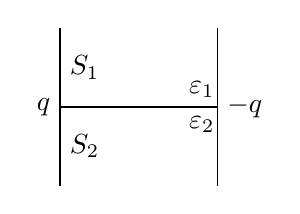
\begin{tikzpicture}
			\draw (0,0) ++ (0,-1) -- ++(0,2);
			\draw (0,0) -- ++ (2,0) ++ (0,-1) -- ++ (0,2);
			\node[left] at (0,0) {$q$};
			\node[right] at (2,0) {$-q$};
			\node[right] at (0,0.5) {$S_{1}$};
			\node[right] at (0,-0.5) {$S_{2}$};
			\node[above] at (1.8,0) {$\varepsilon_{1}$};
			\node[below] at (1.8,0) {$\varepsilon_{2}$};
		\end{tikzpicture}
		\captionof{figure}{}\label{fig:4}
	}
	% \begin{figure}[htbp]
	% 	\centering
	% 	\begin{tikzpicture}
	% 		\draw (0,0) ++ (0,-1) -- ++(0,2);
	% 		\draw (0,0) -- ++ (2,0) ++ (0,-1) -- ++ (0,2);
	% 		\node[left] at (0,0) {$q$};
	% 		\node[right] at (2,0) {$-q$};
	% 		\node[right] at (0,0.5) {$S_{1}$};
	% 		\node[right] at (0,-0.5) {$S_{2}$};
	% 		\node[above] at (1.8,0) {$\varepsilon_{1}$};
	% 		\node[below] at (1.8,0) {$\varepsilon_{2}$};
	% 	\end{tikzpicture}
	% 	\caption{}\label{fig:4}
	% \end{figure}
	\begin{solution}
		在介质分界面上
		\[
			E_{1\mathrm{t}} = E_{2\mathrm{t}}
		\]
		电场强度和电位移矢量均与电介质分界面平行,设 $E_{1} = E_{2} = E$,则
		\begin{align*}
			D_{1} &= \varepsilon_{1} E\\
			D_{2} &= \varepsilon_{2} E
		\end{align*}
		导体表面电荷面密度 $\sigma$ 与该处的电位移矢量 $D$ 相等,故
		\begin{gather*}
			D_{1} S_{1} + D_{2} S_{2} = \sigma_{1} S_{1} + \sigma_{2} S_{2} = q\\
			\varepsilon_{1} S_{1} E + \varepsilon_{2} S_{2} E = q
		\end{gather*}
		故
		\begin{align*}
			E &= \frac{q}{\varepsilon_{1} S_{1} + \varepsilon_{2} S_{2}}\\
			D_{1} &= \frac{\varepsilon_{1} q}{\varepsilon_{1} S_{1} + \varepsilon_{2} S_{2}}\\
			D_{2} &= \frac{\varepsilon_{2} q}{\varepsilon_{1} S_{1} + \varepsilon_{2} S_{2}}
		\end{align*}
	\end{solution}
\end{ti}

\begin{ti}[15 分]
	如图~\ref{fig:5} 所示,试确定浅埋半球接地体的危险半径 $r_0$,设跨步电压安全限值为 $U_0$,入地电流为 $I$,土壤的电导率为 $\gamma$,跨步距离为 $b$。
	\marginpar{%
		\centering
		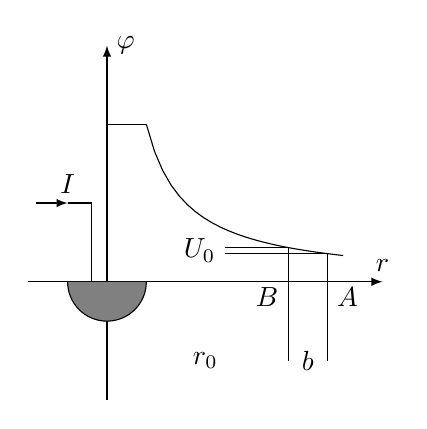
\begin{tikzpicture}[domain=0.5:3]
			\draw[-latex] (-1,0) -- (3.5,0) node[above] {$r$};
			\draw[-latex] (0,-1.5) -- (0,3) node[right] {$\varphi$};
			\filldraw[fill=gray,draw=black] (0.5,0) arc (0:-180:0.5) -- (-0.5,0);
			\draw[-latex] (-0.9,1) -- (-0.5,1) node[above] {$I$};
			\draw (-0.5,1) -- (-0.2,1) -- (-0.2,0);
			\draw (0,2) -- (0.5,2);
			\draw plot (\x,1/\x);
			\draw (1.5,1/2.3) -- (2.3,1/2.3) -- (2.3,-1);
			\draw (1.5,1/2.8) -- (2.8,1/2.8) -- (2.8,-1);
			\node[left] at (1.5,0.39596) {$U_{0}$};
			\node[left] at (2.3,-0.2) {$B$};
			\node[right] at (2.8,-0.2) {$A$};
			\node at (2.55,-1) {$b$};
			\node at (1.25,-1) {$r_{0}$};
		\end{tikzpicture}
		\captionof{figure}{}\label{fig:5}
	}
	% \begin{figure}[htbp]
	% 	\centering
	% 	\begin{tikzpicture}[domain=0.5:3]
	% 		\draw[-latex] (-1,0) -- (3.5,0) node[above] {$r$};
	% 		\draw[-latex] (0,-1.5) -- (0,3) node[right] {$\varphi$};
	% 		\filldraw[fill=gray,draw=black] (0.5,0) arc (0:-180:0.5) -- (-0.5,0);
	% 		\draw[-latex] (-0.9,1) -- (-0.5,1) node[above] {$I$};
	% 		\draw (-0.5,1) -- (-0.2,1) -- (-0.2,0);
	% 		\draw (0,2) -- (0.5,2);
	% 		\draw plot (\x,1/\x);
	% 		\draw (1.5,1/2.3) -- (2.3,1/2.3) -- (2.3,-1);
	% 		\draw (1.5,1/2.8) -- (2.8,1/2.8) -- (2.8,-1);
	% 		\node[left] at (1.5,0.39596) {$U_{0}$};
	% 		\node[left] at (2.3,-0.2) {$B$};
	% 		\node[right] at (2.8,-0.2) {$A$};
	% 		\node at (2.55,-1) {$b$};
	% 		\node at (1.25,-1) {$r_{0}$};
	% 	\end{tikzpicture}
	% 	\caption{}\label{fig:5}
	% \end{figure}
	\begin{solution}
		电流密度
		\[
			J=\frac{I}{2\uppi r^2}
		\]
		则
		\[
			E=\frac{J}{\gamma}=\frac{I}{2\uppi\gamma r^2}	
		\]
		电位
		\[
			\varphi(r)=\int_{r}^{+\infty}E\dd r=\frac{I}{2\uppi\gamma r}
		\]
		跨步电压
		\[
			\varphi(r-b)-\varphi(r)=\frac{bI}{2\uppi\gamma(r-b)r}\approx\frac{bI}{2\uppi\gamma r^2}\xlongequal{\text{令}} U_0
		\]
		解得
		\[
			r_0=\sqrt{\frac{bI}{2\uppi\gamma U_0}}	
		\]
	\end{solution}
\end{ti}

\begin{ti}[10 分]
	如图~\ref{fig:6} 所示,已知无穷长电流和两种媒质的磁导率,求两种媒质中的磁感应强度。
	\marginpar{%
		\centering
		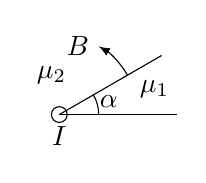
\begin{tikzpicture}
			\draw (0,0) node[below=1pt] {$I$} circle (0.1);
			\draw (0,0) -- ++ (1.5,0);
			\draw (0,0) -- ++ (30:1.5);
			\node at (15:1.25) {$\mu_{1}$};
			\draw (0.5,0) arc (0:30:0.5);
			\node at (15:0.65) {$\alpha$};
			\node at (-0.1,0.5) {$\mu_{2}$};
			\draw[-latex] (30:1) arc (30:60:1) node[left] {$B$};
		\end{tikzpicture}
		\captionof{figure}{}\label{fig:6}
	}
	% \begin{figure}[htbp]
	% 	\centering
	% 	\begin{tikzpicture}
	% 		\draw (0,0) node[below=1pt] {$I$} circle (0.1);
	% 		\draw (0,0) -- ++ (1.5,0);
	% 		\draw (0,0) -- ++ (30:1.5);
	% 		\node at (15:1.25) {$\mu_{1}$};
	% 		\draw (0.5,0) arc (0:30:0.5);
	% 		\node at (15:0.65) {$\alpha$};
	% 		\node at (-0.1,0.5) {$\mu_{2}$};
	% 		\draw[-latex] (30:1) arc (30:60:1) node[left] {$B$};
	% 	\end{tikzpicture}
	% 	\caption{}\label{fig:6}
	% \end{figure}
	\begin{solution}
		根据安培环路定理、媒质分界面的衔接条件
		\[
			\oint_l\vec{H}\bullet\dd l=\oint_{l_1}\frac{\vec{B}}{\mu_1}\dd l+\oint_{l_2}\frac{\vec{B}}{\mu_2}\dd l=B\left(\frac{\alpha r}{\mu_1}+\frac{(2\uppi-\alpha)r}{\mu_2}\right)=I
		\]
		其中 $l$ 为以电流为中心,半径为 $r$ 的圆,$l_1,l_2$ 分别为 $l$ 在媒质 $\mu_1$、$\mu_2$ 中的部分,解得
		\[
			B=\frac{I\mu_1\mu_2}{(\alpha\mu_2+(2\uppi-\alpha)\mu_1)r}
		\]
	\end{solution}
\end{ti}

\begin{ti}[15 分]
	一个球形电容器的内、外半径分别为 $a$ 和 $b$,内、外导体间材料的介电常数为 $\varepsilon$、电导率为 $\gamma$,在内、外导体间加低频电压 $u=U_m\cos\omega t$。求内外导体间的全电流。
	\begin{solution}
		根据高斯通量定理
		\[
			\oiint_{S}\vec{D}\bullet\dd S=4\uppi r^2D=Q
		\]
		其中 $S$ 为球心在球形电容器球心,半径为 $r(a<r<b)$ 的球面,解得
		\[
			E=\frac{D}{\varepsilon}=\frac{Q}{4\uppi\varepsilon r^2}
		\]
		联立
		\[
			\int_{a}^{b}E\dd r=\frac{Q}{4\uppi\varepsilon}\left(\frac{1}{a}-\frac{1}{b}\right)=u=U_m\cos\omega t
		\]
		解得
		\[
			Q=\frac{4\uppi\varepsilon abU_m\cos\omega t}{b-a}
		\]
		则
		\begin{align*}
			J=\gamma E&=\frac{ab\gamma U_m\cos\omega t}{(b-a)r^2}\\
			\frac{\partial D}{\partial t}&=-\frac{\varepsilon\omega abU_m\sin\omega t}{(b-a)r^2}
		\end{align*}
		全电流密度
		\[
			\frac{abU_m}{(b-a)r^2}\left(\gamma\cos\omega t-\varepsilon\omega\sin\omega t\right)
		\]
		全电流
		\[
			\frac{4\uppi abU_m}{b-a}(\gamma\cos\omega t-\varepsilon\omega\sin\omega t)
		\]
	\end{solution}
\end{ti}



% \item (15分)一个球形电容器的内、外半径分别为$a$和$b$,内、外导体间材料的介电常数为$\varepsilon$、电导率为$\gamma$,在内、外导体间加低频电压$u=U_m\cos\omega t$。求内外导体间的全电流。\par
% 解:
\end{document}